\documentclass[
    author={Jacob Daniel Halsey},
    supervisor={Prof. Awais Rashid},
    degree={BSc},
    title={Building a Testbed for Evaluating Privacy Enhancing Technologies  (PETs)},
    subtitle={},
    type={software development},
    year={2021}
]{dissertation}

\usepackage[backend=biber,bibstyle=ieee,citestyle=numeric]{biblatex}
\bibliography{dissertation}

\usepackage{setspace} 
\setstretch{1.25}

\usepackage{subfig}

\usepackage{listings, listings-rust}
\lstset{
	frame=tb,
	language=Rust,
	keywordstyle=\color{blue},
	stringstyle=\color{code-string},
	commentstyle=\color{code-comment},
	tabsize=4,
	basicstyle={\small\ttfamily},
	showstringspaces=false,
	breaklines=true,
	aboveskip=3mm,
	belowskip=0mm,
}

\begin{document}

\maketitle
\frontmatter
\makedecl
\tableofcontents

\chapter*{Executive Summary}

The goal of this project is to produce a simple and lightweight testbed platform for evaluating privacy enhancing
technologies.
It should provide support for testing varied architectures and network topologies, such as client-server and
peer-to-peer applications.
It should also support simulating applications for different types of platforms including mobile phone apps.

\vspace{1cm}

Summary of work:

\begin{itemize}
\item I have developed a flexible command line tool called \emph{kvm-compose} for Linux using the Rust
      language and \emph{libvirt} library for building and destroying virtual testing environments.
\item In the process I have made some contributions to the \emph{libvirt-rust} language
      bindings open source library.
\item I have then implemented some example projects using the testbed tool.
\end{itemize}

\chapter*{Supporting Technologies}

\begin{singlespace}
	\begin{itemize}
		\item \emph{Linux KVM} (Kernel-based Virtual Machine) - \url{https://www.linux-kvm.org/}
		\item \emph{Open vSwitch} Virtual multilayer switch - \url{https://www.openvswitch.org/}
		\item \emph{libvirt} Virtualization API - \url{https://libvirt.org/}
		\item \emph{Rust} Language, Compiler, Toolchain, etc. - \url{https://www.rust-lang.org/}
		\item \emph{libvirt-rust} Rust bindings to the libvirt - \url{https://gitlab.com/libvirt/libvirt-rust}
		\item \emph{clap} Rust command Line Argument Parser - \url{https://github.com/clap-rs/clap}
		\item \emph{serde} Rust Serialization framework - \url{https://github.com/serde-rs/}
		\item \emph{serde-yaml} YAML backend for serde - \url{https://github.com/dtolnay/serde-yaml}
		\item \emph{serde-plain} Plain text backend for serde - \url{https://github.com/mitsuhiko/serde-plain}
		\item \emph{thiserror} Rust error derive macro - \url{https://github.com/dtolnay/thiserror}
		\item \emph{anyhow} Rust error handling framework - \url{https://github.com/dtolnay/anyhow}
		\item \emph{simple\_logger} Rust logging implementation - \url{https://github.com/borntyping/rust-simple_logger}
		\item \emph{xml-rs} XML library for Rust - \url{https://github.com/netvl/xml-rs}
		\item \emph{validator} Rust struct validation - \url{https://github.com/Keats/validator}
		\item \emph{directories} User data directories library - \url{https://github.com/dirs-dev/directories-rs}
		\item \emph{reqwest} Rust HTTP Client - \url{https://github.com/seanmonstar/reqwest}
		\item \emph{indicatif} Rust command line progress indicator - \url{https://github.com/mitsuhiko/indicatif}
		\item \emph{tempfile} Rust temporary file library - \url{https://github.com/Stebalien/tempfile}
		\item \emph{casual} Rust user input parser - \url{https://github.com/rossmacarthur/casual}
		\item \emph{derive-new} Rust new constructor macro - \url{https://github.com/nrc/derive-new}
		\item \emph{enum-iterator} Rust macro for iterating enums - \url{https://github.com/stephaneyfx/enum-iterator}
		\item \emph{rust-embed} Embeds files into Rust binaries - \url{https://github.com/pyros2097/rust-embed}
	\end{itemize}
\end{singlespace}

\chapter*{Acknowledgements}

I would like to thank my supervisor Professor Awais Rashid and co-supervisor Joe Gardiner for their
project proposal and support and guidance in completing it.

\mainmatter


\chapter{Contextual Background}
\label{chap:context}

The UK Research and Innovation (UKRI) is a non-departmental public body of the United Kingdom Government
sponsored by the Department for Business, Energy and Industrial Strategy~\cite{ukri_who_we_are}.
In October 2020 the UKRI announced the creation of the National Research Centre on Privacy, Harm Reduction
and Adversarial Influence Online (REPHRAIN)~\cite{ukri_new_centre}.
The centre is made up of researchers in computer science, international relations, law, psychology, management,
design, digital humanities, public policy, political Science, criminology, and sociology from five British
universities including the University of Bristol. \\

REPHRAIN should be understood in the context of the UK government's \emph{Online Harms White Paper} public
consultation beginning in April 2019~\cite{uk_gov_online_harms}, which sets out plans for new online safety 
measures; REPHRAIN's missions and outcomes are aligned with this paper~\cite{rephrain_harms}. \\

REPHRAIN will focus on three core missions~\cite{rephrain_missions}:

\begin{enumerate}
	\item Delivering privacy at scale while mitigating its misuse to inflict harms.
	\item Minimising harms while maximising benefits from a sharing-driven digital economy.
	\item Balancing individual agency vs. the social good.
\end{enumerate}

The three missions will require looking at Privacy Enhancing Technologies (PETs); including their capabilities,
applications of PETs in addressing existing online harms, mitigating the potential abuse of PETs, embedding the PETs
into infrastructures, and developing new PETs.
In order to facilitate this REPHRAIN intends to build a toolbox of resources including a PETs testbed. The testbed
will be used researchers in developing, testing, and evaluating the PETs. The aim of this project is to develop
a prototype for this testbed.

\section{What are Privacy Enhancing Technologies (PETs)?}

Before we discuss Privacy Enhancing Technologies we must consider what we mean by "privacy". REPHRAIN is 
primarily using the definitions set out by D. J. Solove in his
2006 article \emph{A Taxonomy of Privacy}~\cites{solove_privacy}{rephrain_harms}. Solove notes that the
definition of privacy has often been very broad or vague, and therefore sets out to develop
a taxonomy of privacy violations. He has defined four groups of harmful activities (See figure~\ref{privacy_taxonomy}). \\

\begin{figure}
\centering
\parbox{7cm}{
	\begin{enumerate}
		\item Information collection
		\begin{enumerate}
			\item Surveillance
			\item Interrogation 
		\end{enumerate}
		\item Information processing
		\begin{enumerate}
			\item Aggregation
			\item Identification
			\item Insecurity
			\item Secondary Use
			\item Exclusion
		\end{enumerate}
	\end{enumerate}
}
\qquad
	\begin{minipage}{7cm}
		\begin{enumerate}
			\setcounter{enumi}{2}
			\item Information  dissemination
			\begin{enumerate}
				\item Breach of Confidentiality
				\item Disclosure
				\item Exposure
				\item Increased Accessibility
				\item Blackmail
				\item Appropriation
				\item Distortion
			\end{enumerate}
			\item Invasion
			\begin{enumerate}
				\item Intrusion
				\item Decisional Interference
			\end{enumerate} 
		\end{enumerate}
	\end{minipage}
	\caption{A Taxonomy of Privacy Violations~\cite{solove_privacy}.}
	\label{privacy_taxonomy}
\end{figure}

Broadly speaking a Privacy Enhancing Technology is any solution or approach in hardware or software that helps
protect a user from such privacy violations~\cite{buckley_pets}. Some examples of PETs could include 
Onion routing such as the Tor network (which enables anonymous communication), or
end-to-end encrypted messaging systems such as the Signal protocol. 
Kaaniche et al.~\cite{kaaniche_2020_privacy} have defined a more comprehensive classification of PETs
 (see Figure~\ref{pet_taxonomy}).

\begin{figure}
	\centering
	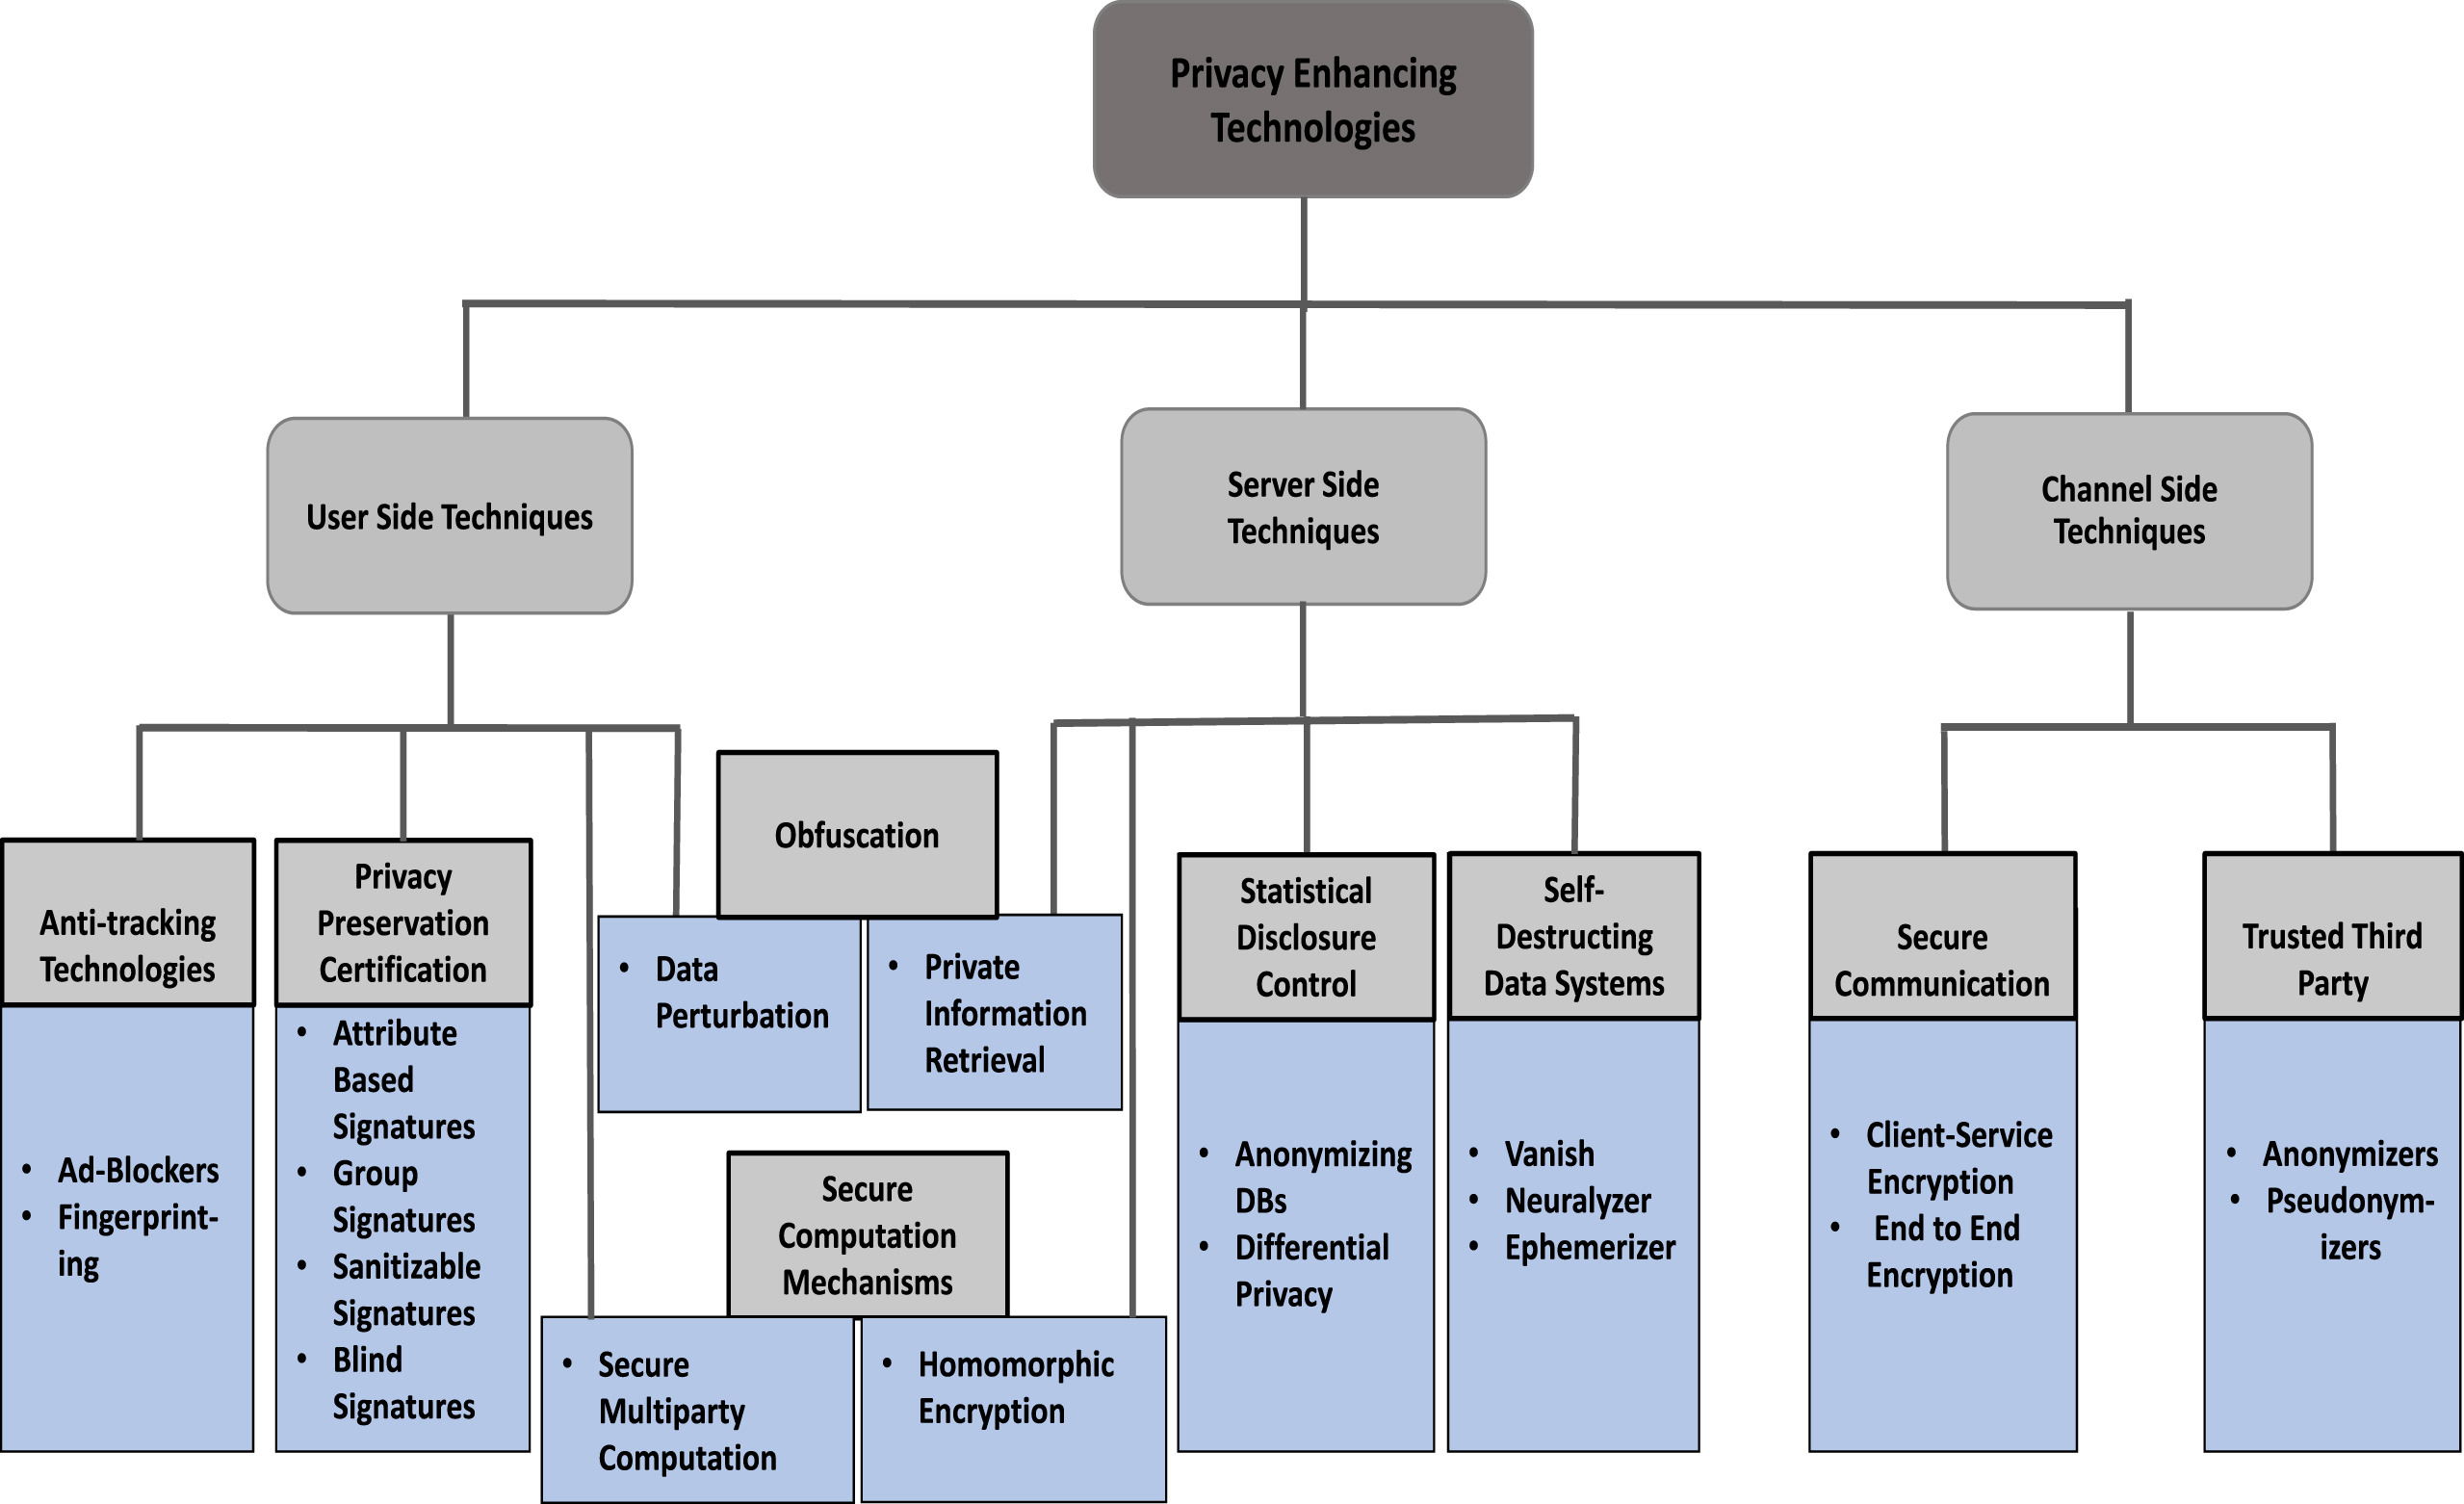
\includegraphics{img/pet_taxonomy}
	\caption{A Taxonomy of privacy enhancing technologies~\cite{kaaniche_2020_privacy}.}
	\label{pet_taxonomy}
\end{figure}

\section{Existing Solutions}

There has been some existing research by Tekeoglu and Tosun~\cite{tekeoglu_2016_testbed} who have developed 
a privacy testbed for Internet-of-Things (IoT) devices. Their approach has some similar goals to this project 
in that it looks at capturing layer 2 and 3 network traffic. They note that the testbed enables experiments such
as port vulnerability scans, checking what cipher suites are used (or not), and generally monitoring 
network traffic to see what data is being collected. However their testbed is different in that it is only designed
for IoT devices; rather than general purpose PET applications.

\section{High Level Objectives}

Overall the high-level objective of this project is to develop a simple and lightweight
testbed platform for evaluating PETs:

\begin{itemize}
	\item The testbed should support testing various architectures and network topologies, 
	including client/server and peer-to-peer applications, to accommodate a variety of PETs.
	\item The testbed must be able to collect information such as packet captures
	for use in evaluating the privacy properties.
	\item The testbed should support different platforms such as desktop and mobile apps,
	and both applications where the source code is available or only pre-built binaries.
	\item The testbed should enable a high level of automation, such that working with large test
	environments because feasible, and the setup can easily and programmatically be replicated.
\end{itemize}

\chapter{Technical Background}
\label{chap:technical}

In this chapter I will discuss some of the technologies which this project depends or builds upon.

\section{Virtualization}

\begin{quotation}
	`Virtualization uses software to create an abstraction layer over computer hardware that allows the hardware 
	elements of a single computer—processors, memory, storage and more—to be divided into multiple virtual computers, 
	commonly called virtual machines (VMs). Each VM runs its own operating system (OS) and behaves like an independent 
	computer, even though it is running on just a portion of the actual underlying computer hardware.'~\cite{ibm_virtualization}
\end{quotation}

Virtualization\footnote{I am a British citizen, and this is a dissertation at a British university, 
and therefore I am very much aware that the correct spelling in British English is `virtualisation', however the
majority of platforms, libraries, and sources I will be referencing use the US English spelling, 
so I have chosen to do the same. }
 will therefore be a very useful technology for the testbed, since it will allow us to model
an environment consisting of multiple computers such as application clients and servers, and run
them all within a single machine. In addition, modern CPU extensions (such as Intel VT and AMD-V) 
provide hardware-assisted / accelerated virtualization support, allowing the virtual machines to 
have near native performance which will help in meeting the goal of minimal overhead for the testbed. \\

In order to use virtualization a \emph{Hypervisor} is required, this is the software layer sits between
the physical hardware and manages the virtual machines. A hypervisor may run directly on the physical machine
in place of a conventional operating system - as a Type 1 or \emph{bare-metal} hypervisor,
or run within a separate host operating system - as a Type 2 or \emph{hosted} hypervisor. \\

\subsection{KVM}
\label{subsect:kvm}

For the prototype testbed I will be using \emph{Kernel-based Virtual Machine} (KVM), which is a 
kernel module for the Linux operating system that allows it to function as a hypervisor. 
The advantage is that KVM (and the Linux kernel itself) are free and open-source software 
under GNU licenses, and it is a stable and mature platform~\cite{redhat_kvm}.
In userspace QEMU\footnote{Note QEMU can also function as its own independent type 2 hypervisor 
	but KVM is required to enable hardware acceleration,
see \url{https://www.packetflow.co.uk/what-is-the-difference-between-qemu-and-kvm/}}
may then use KVM to provide a full virtualization platform. \\

\emph{libvirt} is an open-source toolkit for managing virtualization platforms~\cite{libvirt},
it supports QEMU/KVM as well as hypervisors from other vendors. It is written in C, 
with bindings available in many other programming languages, making it a suitable library for developing 
the testbed. Support for other platforms also means it would be easier to add support
for additional hypervisors in future.

\section{Containerization}

Having discussed full platform / machine virtualization it is worth also mentioning containerization
which is an alternative lightweight approach to virtualizing applications. In particular 
there is the Docker platform for Linux containers which has become very popular in recent
years~\cite{zdnet_docker_2018}. \\

\begin{figure}
	\centering
	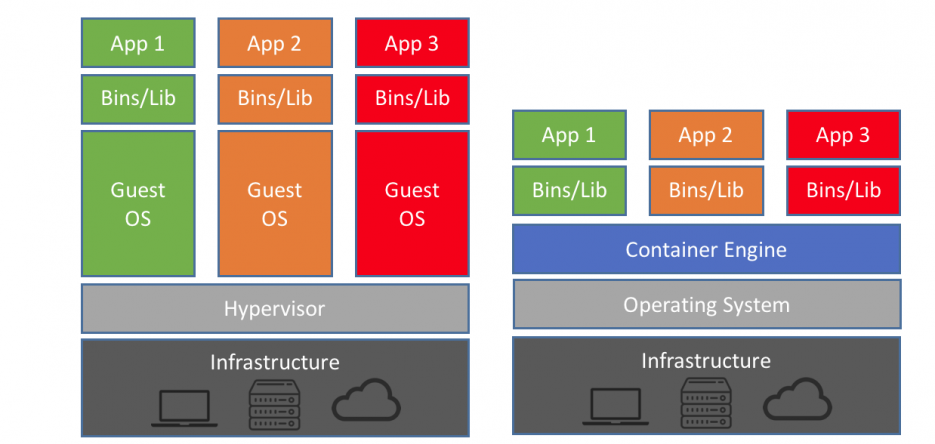
\includegraphics[width=12cm]{img/containers}
	\caption[]{Platform Virtualization vs Containerization\footnotemark}
	\label{containers_diagram}
\end{figure}
\footnotetext{Graphic from \url{https://blog.netapp.com/blogs/containers-vs-vms/}}

Unlike full platform virtualization, containerization does not virtualize a whole computer 
(or require hardware acceleration), instead it uses namespacing within the host operating 
system kernel to create an isolated environment. This has many practical uses, making deploying
software and services very quick and easy, but unfortunately it is not ideal for our testbed, since
it would mean all applications would have to use the same operating system; it couldn't be 
used to simulate different platforms. \\

While I will not be using containerization, the \emph{Docker Compose} tool~\cite{docker_compose}
used for orchestrating containers has provided some useful inspiration for the testbed.
\emph{Docker Compose} is a command line program with two core subcommands \emph{up}
and \emph{down} which are used to either build or destroy a set of containers as defined
in a YAML configuration file. The configuration file may define a list of containers, each 
with options including an image to download, an entry command to run, volumes to attach,
and environment variables, the config may also define virtual networks and attach them
to the containers. These are all very useful features in line with the goals for the testbed, and as such
I will try to replicate them but within a fully virtualized environment (QEMU/KVM).

\section{Virtual Networks}

\subsection{Software Defined Networking}

\section{The Rust Language}

As you will see in Chapter~\ref{chap:execution}, I have chosen to use the Rust programming
language for developing the testbed. Although there are no doubt many languages which
could have been used, I will provide some background on Rust, and its advantages for this
project. \\

Rust is a modern systems programming language, originally developed by Mozilla, 
with its first stable release in 2015. It is designed with a focus on performance, safety
and concurrency. \\

\begin{singlespace}
	It has some key advantages:
	\begin{itemize}
		\item Excellent performance; on par with
		 C/C++\footnote{\url{https://benchmarksgame-team.pages.debian.net/benchmarksgame/index.html}}.
		\item Easy interaction with C libraries via FFI, making 
		the \emph{libvirt}~\cite{libvirt_rust} bindings possible.
		\item A simple to use package manager - \emph{Cargo}, along with a rich ecosystem of 
		libraries\footnote{\url{https://crates.io/}}.
		\item Modern functional constructs such as sum types and pattern matching.
		\item Memory and thread safety are enforced at compile time~\cite{systems_rust}.
		\item The compiler and standard library support a large number of platforms.
	\end{itemize}
\end{singlespace}

\section{Cloud Init}


\chapter{Project Execution}
\label{chap:execution}

\section{Modifications to \emph{libvirt-rust}}

As mentioned in section \ref{subsect:kvm} I was going need to use the \emph{libvirt} library for interacting
with QEMU/KVM, as well as the bindings to access it from the Rust language: \emph{libvirt-rust}~\cite{libvirt_rust}.
During my initial experiments developing the project I discovered that under certain build setups / toolchains
the \emph{libvirt-rust} crate\footnote{Rust packages such as libraries, managed through the \emph{Cargo} package
manager are known as `Crates'}
failed to compile, due to it containing function declarations that did not actually exist in the \emph{libvirt}
library. This is described in full detail in my issue
report: \url{https://gitlab.com/libvirt/libvirt-rust/-/issues/1}.\\

I submitted a fixed version of \emph{libvirt-rust} with these invalid functions removed, but also with
a test case that builds the bindings in a static library, therefore checking that all the symbols (such as
functions) did actually exist in the underlying \emph{libvirt} library. 
The tests are automatically run as part of the 
CI/CD pipeline so this sort of problem should be prevented in future. The merge request was approved by
the project maintainers: \url{https://gitlab.com/libvirt/libvirt-rust/-/merge_requests/14}. \\

Whilst working with \emph{libirt} I also discovered that I was receiving duplicate error messages printed
to the console (via \emph{stdout/stderr}), this was because by default \emph{libvirt} has an error handler
configured to print all errors, but at the same time the \emph{libvirt-rust} binding functions also returned
a \lstinline|Result<_, virt::error::Error>| type (the idiomatic approach in Rust), 
which on failure I was also printing to the console
via the logging framework. So I also added a \lstinline|clear_error_func()| that binds to \lstinline|virSetErrorFunc|
along with my changes, so that the default error handler can be disabled.

\section{\emph{kvm-compose}}

\section{Examples}

\section{Development Practice}

During development I used the \emph{Git} version control system, with free hosting from \emph{GitHub Inc}.
I also made use of the \emph{GitHub Actions} CI/CD platform, with a workflow configured to check that
the project builds and passes style checks on each push to the repository.

\chapter{Critical Evaluation}
\label{chap:evaluation}

{\bf A topic-specific chapter, of roughly $15$ pages} 
\vspace{1cm} 

\noindent
This chapter is intended to evaluate what you did.  The content is highly 
topic-specific, but for many projects will have flavours of the following:

\begin{enumerate}
\item functional  testing, including analysis and explanation of failure 
      cases,
\item behavioural testing, often including analysis of any results that 
      draw some form of conclusion wrt. the aims and objectives,
      and
\item evaluation of options and decisions within the project, and/or a
      comparison with alternatives.
\end{enumerate}

\noindent
This chapter often acts to differentiate project quality: even if the work
completed is of a high technical quality, critical yet objective evaluation 
and comparison of the outcomes is crucial.  In essence, the reader wants to
learn something, so the worst examples amount to simple statements of fact 
(e.g., ``graph X shows the result is Y''); the best examples are analytical 
and exploratory (e.g., ``graph X shows the result is Y, which means Z; this 
contradicts [1], which may be because I use a different assumption'').  As 
such, both positive {\em and} negative outcomes are valid {\em if} presented 
in a suitable manner.

\chapter{Conclusion}
\label{chap:conclusion}

{\bf A compulsory chapter,     of roughly $5$ pages} 
\vspace{1cm} 

\noindent
The concluding chapter of a dissertation is often underutilised because it 
is too often left too close to the deadline: it is important to allocation
enough attention.  Ideally, the chapter will consist of three parts:

\begin{enumerate}
\item (Re)summarise the main contributions and achievements, in essence
      summing up the content.
\item Clearly state the current project status (e.g., ``X is working, Y 
      is not'') and evaluate what has been achieved with respect to the 
      initial aims and objectives (e.g., ``I completed aim X outlined 
      previously, the evidence for this is within Chapter Y'').  There 
      is no problem including aims which were not completed, but it is 
      important to evaluate and/or justify why this is the case.
\item Outline any open problems or future plans.  Rather than treat this
      only as an exercise in what you {\em could} have done given more 
      time, try to focus on any unexplored options or interesting outcomes
      (e.g., ``my experiment for X gave counter-intuitive results, this 
      could be because Y and would form an interesting area for further 
      study'' or ``users found feature Z of my software difficult to use,
      which is obvious in hindsight but not during at design stage; to 
      resolve this, I could clearly apply the technique of Smith [7]'').
\end{enumerate}

\backmatter
\printbibliography

\end{document}
